% ------------- START PREAMBLE --------------------
\documentclass[12pt]{report}
\usepackage[utf8]{inputenc}
\usepackage[left=2.5cm,right=2cm,top=2cm,bottom=2.5cm]{geometry}
\usepackage{titlesec}
\newcommand{\sectionbreak}{\clearpage}  % Start new page with each section
\titleformat{\chapter}[hang]{\normalfont\huge\bfseries}{\chaptertitlename\ \thechapter:}{1em}{} % Chapter number and name on same line
\usepackage{graphicx}                                                                           % Implement images
\usepackage[hidelinks]{hyperref}                                                                           % Make content of table clickable and remove red boxes around links (hidelinks)
\usepackage{color}
\usepackage{graphicx}
\usepackage{biblatex}                                                                           % Bibliography
\addbibresource{resources/bibliography.bib}                                                               % Specify .bib database
\usepackage[usenames,dvipsnames,svgnames,table]{xcolor}
\usepackage{url}
\usepackage{titlepic}       %Graphics in frontpage
\usepackage[acronym,toc]{glossaries} % Packet for acronyms
\usepackage{imakeidx}       % Indices - alphabetic list of main terms
\makeindex[columns=2, title=Index, options= -s resources/index-style.ist]
\usepackage{changepage}     % used to adjust indentation on subsections
\usepackage{titlesec}       % add subsection inside subsections (e.g. 2.1.1)
\usepackage{datetime}       % insert date automatically (used in the title page)
\newdateformat{monthyeardate}{%
                                \monthname[\THEMONTH] \THEYEAR}



% ------------- END PREAMBLE --------------------


%----------------------ACRONYMS
\makeglossaries
\newacronym{rom}{ROM}{Read Only Memory}

\newacronym{bios}{BIOS}{Basic Input Output System}

\newacronym{api}{API}{Application Programming Interface}

\newacronym{ssl}{SSL}{Secure Socket Layer}

\newacronym{ssh}{SSH}{Secure Shell}

\newacronym{dhcp}{DHCP}{Dyanmic Host Configuration Protocol}

\newacronym{dns}{DNS}{Domain Name System}


%################# BEGIN DOCUMENT ######################
\begin{document}

%---------------------------TITLEPAGE(Blank)
\begin{titlepage}
\title{\textbf{The Dictionary \\ About \\ (Almost) \\ Everything} }
\titlepic{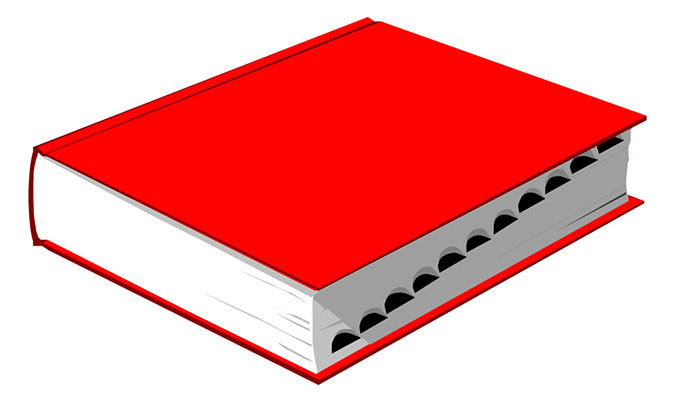
\includegraphics[width=8cm]{resources/dict.jpg}}
\author{\textit{Piraveen Perinparajan}}
\date{\monthyeardate\today}
\end{titlepage}
\maketitle



%---------------------------PREFACE
\chapter*{Preface}  % the asterix prevents numbering of preface chapter
Especially for beginners, learning a new topic in any area can be overwhelming. This document seeks to solve this by providing real world examples to basic and intermediate level terms (in each respective topic) whenever possible. \\

\noindent The idea is to provide definitions for common words and terms in software engineering, artificial intelligence, cryptography, mathematics and physics - in Layman's terms. This is a document that is meant to be understood by everyone. Ambitious? Indeed. Currently the main focus is software engineering, artificial intelligence and cryptography. \\



\noindent This project started in January 2017. \\
\noindent Feel free to contribute.\\

\noindent Happy reading! \\

\noindent \textit{Piraveen Perinparajan}


%-----------------------TABLE OF CONTENTS
\addcontentsline{toc}{chapter}{Preface} %Add preface to list of contents
\clearpage
    \tableofcontents
\clearpage


\printglossary[title=Acronyms,type=\acronymtype]   % Print glossary after ToC
\printglossary

% Set vertical spacing
\setlength{\parskip}{1.5em}   % length between each paragraph
\setlength\parindent{0pt}   % no indentation after each paragraph for whole file


%---------------------------Computer Science Chapter
\chapter{Computer Science}

\section{Basic}
\textbf{Firmware\index{firmware} \\}
Firmware is software that is semi-permanently placed in hardware. Firmware does not disappear when 
hardware is turned off (typically stored in Flash or \acrshort{rom}). 
Firmware is typically involved with very basic low-level operations, which without a device, would be
non-functional.  

\textbf{BIOS\index{BIOS}} \\
\acrfull{bios} is a software that is saved on the computer's motherboard
and is turned on whenever the computer boots up. Its primary task is to prepare the components of the machine, so that other software (like the operating system) can boot up, run and take over the control of the machine.  

\textbf{Modular\index{modular}} \\
Refers to the design of any system composed of separate components that can be connected together. The beauty of modular architecture is that you can replace or add any one component (module) without affecting the rest of the system. The opposite of a modular architecture is an integrated architecture, in which no clear divisions exist between components. The term modular can apply to both hardware and software. Modular software design, for example, refers to a design strategy in which a system is composed of relatively small and autonomous routines that fit together. 

\textbf{Standalone application\index{standalone application}} \\
A standalone application is a application that is downloaded on your local computer and is self contained. Meaning it's not dependent on another service for it to run, unlike an web application that requires a web browser to work. (i.e. you need Chrome/Safari/Firefox to run Facebook). 

\newpage
    



\section{Cybersecurity}

\textbf{Botnet} \index{botnet}  \cite{cybersecurity:botnets} \\
A botnet is different from a isolated machine with malware. A botnet is a collection of infected machines which are coordinated through a central server called the Command \& Contrtrol server, C\&C server. The users of the machines involved in a botnet isn't necessarily aware that they're a part of the botnet.  A classic example for which a botnet can be used is a DDoS attack (hence the D in Distributed).  

\textbf{Steganography} \url{https://www.youtube.com/watch?v=TWEXCYQKyDc} 





\section{Networking}
    \begin{adjustwidth}{2.5em}{0cm}
    %\parskip{5cm}   % length between each paragraph
    \parindent{.}   % no indentation after each paragraph for whole file

    %``````` APPLICATION LAYER ```````

    \subsection{Application layer}
    \textbf{DHCP\index{DHCP}} \\
    \acrfull{dhcp} is a network protocol responsible for assigning IP addresses to hosts on a network. The host sends out a broadcast and gets an answer from all the DHCP-servers nearby. It's then up to the host to choose one server and then inform all the other servers which one it chose. Considering the host is IP-less the packet is broadcasted with \textit{UDP}. A DHCP server is often found integrated inside a \textit{router}. 

    
    \textbf{DNS}    \\
    \acrfull{dns} translates an \textit{IP-address} to a website. \\
    Example: For instance, YouTube's IP address is 216.58.209.142. Without DNS you would have to type in the IP-address, instead of youtube.com.  

    
    
    \textbf{SSH\index{SSH}} \\
    \acrfull{ssh} is a cryptographic network protocol used over unsecured networks. It's commonly used to perform remote login on a machine. 
    \end{adjustwidth}
    
    \begin{adjustwidth}{2.5em}{}
    %``````` TRANSPORT LAYER ```````
    \subsection{Transport layer}
    \textbf{TCP} \\
    
    \textbf{UDP} \\
    \end{adjustwidth}
    
    %``````` NETWORK LAYER ```````
    \subsection{Network layer}
    \textbf{IP address} \\
    
    \textbf{ICMP} \\
    
   \textbf{Routing table} \\
   
    
    
    %``````` LINK LAYER ```````
    \subsection{Link layer}
    \textbf{ARP} \\
    
    \textbf{MAC address} \\
    
    \textbf{PPP} \\
    





\textbf{Firewall} \\

\textbf{FTP} \\


\textbf{Tor} \\





\newpage


\section{Software development}
\setcounter{secnumdepth}{3}

% -------------------
% General
\subsection{General}

\textbf{Abstraction layer}
\textit{Empty.}

\textbf{Async/await}
\textit{Empty.}

\textbf{Binary file\index{binary file}} \\
\textit{Binary means executable code that can be run directly by the machine without the need to be compiled.}

\textbf{Dependency Injection}
\textit{Empty.}

\textbf{Docker (program) \index{Docker}} \\
Docker is a tool designed to make it easier to create, deploy, and run applications by using containers. Containers allow a developer to package up an application with all of the parts it needs, such as libraries and other dependencies, and ship it all out as one package. By doing so, thanks to the container, the developer can rest assured that the application will run on any other machine regardless of any customized settings that machine might have that could differ from the machine used for writing and testing the code.

\textbf{Framework\index{framework}} \\
\textit{Empty.}

\textbf{Git\index{git}} \\
Git is a version control system. 

\textbf{Native language\index{native language}} \\
\textit{A native programming language is compiled to machine code. This is code that's unique to a particular operating system and can only be executed in the environment for which it was compiled. As a result, when you're dealing with a native language you have to have a different compiler for each operating system. You'll have one compiler application for Windows, another one for Mac, another one for a distinct flavor of Linux, and so on. Example of native languages: C, C++, Objective-C }

\textbf{Managed languages\index{managed language}} \\
\textit{In contrast, managed languages are compiled to an intermediate format that works across operating systems. Typically, these languages are compatible across operating systems, and include languages such as C\# and Java. In addition, in manages languages, memory is allocated dynamically at runtime which means the programmer don't need to worry about allocationg and deallocating memory, which is periodically done by the garbage collector. }

\textbf{Modular\index{modular}} \\
Refers to the design of any system composed of separate components that can be connected together. The beauty of modular architecture is that you can replace or add any one component (module) without affecting the rest of the system. The opposite of a modular architecture is an integrated architecture, in which no clear divisions exist between components. The term modular can apply to both hardware and software. Modular software design, for example, refers to a design strategy in which a system is composed of relatively small and autonomous routines that fit together. 

\textbf{Wrapper\index{wrapper}} \\
\textit{In the context of software engineering, a wrapper is defined as an entity that encapsulates and hides the underlying complexity of another entity by means of well-defined interfaces.}


\textbf{Wrapper application\index{wrapper application}} \\
\textit{A wrapper can be a piece of software that provides compatibility layer to another piece of software.}

\textbf{Wrapper function\index{wrapper function}} \\
\textit{A wrapper function is a function that exists for the sole purpose of calling another function.}


\textbf{Web application}
A self-contained web application is a standalone web application; in contrast to a multi-paged website.

\textbf{Scrum}
\textit{Empty.}

\textbf{Kanban}
\textit{Empty.}

\textbf{SQL \index{SQL}} \\
\acrfull{sql} is a language used in programming to manage data in a \acrfull{rdbms}.

\textbf{MySQL \index{MySQL}} \\
MySQL is a SQL-based RDBMS. This means that MySQL uses SQL as a query language to perform the necessary queries. In a relational database, such as MySQL, every table is connected to some other table through relations. 


\begin{table}[!htb]
    \caption{Relation between a person and a car}
    \begin{minipage}{.5\linewidth}
      \centering
        \begin{tabular}{|l|}
            \hline
            \textbf{Person} \\ \hline
            Name            \\ \hline
            Age             \\ \hline
        \end{tabular}
    \end{minipage}%
    \begin{minipage}{.5\linewidth}
      \centering
        \begin{tabular}{|l|}
            \hline
            \textbf{Car}    \\ \hline
            Model            \\ \hline
            Year             \\ \hline
            Owner             \\ \hline
        \end{tabular}
    \end{minipage} 
\end{table}

For instance, these tables may be connected like this: A person may have many cars - but one car only has one owner. 

\textbf{NoSQL \index{NoSQL}} \cite{software:NoSQL} \\
In contrast to MySQL, NoSQL is a database system where the data isn't structured in relations. Instead, everything is stored as key-value pairs inside one single document. A key-value pair may contain a string, integer, an array or a object that holds even more key-value pairs. 

\textbf{MongoDB} \cite{software:MongoDB} \\
\textit{Empty.}


\textbf{Driver} \\
Source: \url{https://www.youtube.com/watch?v=t-aRlwLI-b0}

\clearpage
% --------------------------------------------------------------------------------------
%                                       .NET 
\subsection{.NET}

\textbf{ASP.NET} \\
\textit{Empty.}


\textbf{Common Language Runtime \index{Common Language Runtime}\cite{software:CLR}} \\
The common language runtime manages memory, thread execution, code execution, code safety verification, compilation, and other system services. 
The managed environment of the runtime also eliminates many common software issues. For example, the runtime automatically handles object layout and manages references to objects, releasing them when they are no longer being used. This automatic memory management resolves the two most common app errors, memory leaks and invalid memory references.
The runtime is designed to enhance performance. Although the common language runtime provides many standard runtime services, managed code is never interpreted. A feature called just-in-time (JIT) compiling enables all managed code to run in the native machine language of the system on which it's executing.

\textbf{.NET Framework \index{n@.NET Framework} \cite{software:.net}} \\
The .NET Framework is a managed execution environment that provides a variety of services to its running apps. It consists of two major components: the common language runtime (CLR), which is the execution engine that handles running apps, and the .NET Framework Class Library, which provides a library of tested, reusable code that developers can call from their own apps. The services that the .NET Framework provides to running apps include the following:
\begin{itemize}
    \item \textbf{Memory management.} In many programming languages, programmers are responsible for allocating and releasing memory and for handling object lifetimes. In .NET Framework apps, the CLR provides these services on behalf of the app.
    
    \item \textbf{A common type system.} In traditional programming languages, basic types are defined by the compiler, which complicates cross-language interoperability. In the .NET Framework, basic types are defined by the .NET Framework type system and are common to all languages that target the .NET Framework.

     \item \textbf{An extensive class library.} Instead of having to write vast amounts of code to handle common low-level programming operations, programmers use a readily accessible library of types and their members from the .NET Framework Class Library.

     \item \textbf{Development frameworks and technologies.} The .NET Framework includes libraries for specific areas of app development, such as ASP.NET for web apps, ADO.NET for data access, and Windows Communication Foundation for service-oriented apps.

     \item \textbf{Language interoperability.} Language compilers that target the .NET Framework emit an intermediate code named Common Intermediate Language (CIL), which, in turn, is compiled at runtime by the common language runtime. With this feature, routines written in one language are accessible to other languages, and programmers focus on creating apps in their preferred languages.
\end{itemize}

\textbf{.NET Framework Architecture\index{n@.NET Framework Architecture}} \\
.NET is a software framwork developed by Microsoft that runs primarily on Windows.
It includes a large class library named Framework Class Library (FCL) and provides language interoperability (you can write some pieces of your application in Visual Basic, others in C\# and others in another language - and they can all communicate with each other). Programs written for .NET Framework execute in a software environment named Common Language Runtime (CLR), an application virtual machine that provides services such as security, memory management, and exception handling. (As such, computer code written using .NET Framework is called "managed code".) FCL and CLR together make up the .NET Framework.

\textbf{.NET Core\index{n@.NET Core}} \cite{software:NETCore} \\
.NET Core is a general purpose, modular, cross-platform and open source implementation of the .NET Standard. It contains many of the same APIs as the .NET Framework (but .NET Core is a smaller set) and includes runtime, framework, compiler and tools components that support a variety of operating systems and chip targets. Here are the main characteristics of .NET Core: 
\begin{itemize}
    \item \textbf{Cross-platform:} .NET Core provides key functionality to implement the app features you need and reuse this code regardless of your platform target. It currently supports three main operating systems: Windows, Linux and macOS. You can write apps and libraries that run unmodified across supported operating systems. 
    
    \item \textbf{Open source:} .NET Core is one of the many projects under the stewardship of the .NET Foundation and is available on GitHub. 
    
   \item \textbf{Modular:} .NET Core is modular because it's released through NuGet in smaller assembly packages. Rather than one large assembly that contains most of the core functionality, .NET Core is made available as smaller feature-centric packages. This enables a more agile development model for us and allows you to optimize your app to include just the NuGet packages you need. The benefits of a smaller app surface area include tighter security, reduced servicing, improved performance, and decreased costs in a pay-for-what-you-use model.
\end{itemize}







\textbf{.NET Runtime \index{n@.NET}} \\
\textit{Empty.}


\textbf{.NET Standard} \\
\textit{Empty.}



\section{Hardware}

\textbf{\acrfull{cpu} \index{CPU}} \\
\acrfull{cpu} is often referred to as the brain of the computer - with good reason. The CPU is meant to take care of a variety of tasks, very fast. 

\textbf{Motherboard \index{motherboard}} \\
The motherboard is the most important circuit board on a computer. Every major component is connected to the motherboard. This includes the CPU, GPU, sound card, RAM sticks. The motherboard also houses the BIOS tasked with starting up the computer. 

\textbf{GPU / Video card\index{GPU}\index{video card}} \\
While the CPU is meant to take care of a variety of tasks, the \acrfull{gpu} has one task - to render graphics by performing several mathematical operations alongside the CPU.  

\textbf{RAM \index{RAM}} \\
\acrfull{ram} contains the data required for the CPU to run a specific process (or several processed, depending on the size of the RAM). RAM is faster than your classical hard drive, but has less storage space. It is slower than the CPU's cache, but offers more space. 

\textbf{VRAM \index{VRAM}} \\
Video RAM is Video RAM. Just as the RAM feeds the CPU with data, the VRAM is tasked with feeding the GPU with data so images can be rendered to the screen. The data inside the VRAM is typically textures, frame buffers, shadow maps, bump maps and lightning. 

\textbf{Hard drive} \\

\textbf{SSD} \\

\textbf{Sound card}

\textbf{Router \index{router}} \\
A router is the traffic controller between your own home and the rest of the world. 

\textbf{Modem \index{modem}} \\
The data that get to your house through the cables are analog. A modem converts that signal to digital signals then passes it on to the router that figures out who the data was meant for and sends it their way. 

\textbf{Hotspot (WiFi)} \\




\newpage

\section{Web}

\subsection{General}
\textbf{API\index{API}} \\
API stands for Application Programming Interface. It's a way to let one application talk to another application through a middle-man - the API. 

\textbf{RESTAPI} \\
API stands for Application Programming Interface. It's a way to let one application talk to another application through a middle-man - the API. 

\textbf{Transpile\index{transpile}} \\
In the context of web, transpiling means transforming one script into another script. A good example would be what Babel does when developing with react - it transpiles the JavaScript from ECMAScript 6 to ES5. One might be tempted to think that from for instance C\# to IL is called transpiling. This would be wrong because the two languages have very different levels of abstraction (complexity). 

\textbf{TLS} \\ 
Transport Layer Security is an extra layer between the TCP and HTTP layer, that together forms the HTTPS protocol. The TLS does an extra step of authentication before the browser starts to recieve data from the server. During this step the TLS will check if the connected server is actually the server we want to connect to. \cite{web:ssl}


\textbf{Onion web/onion browser\index{onion web}} \\
It's called the onion web because when a request is made on the Tor-network (using onion) every request that is sent out from your computer is wrapped up in several layers of encryption - kind of like an onion. So as that request travels through multiple computers, every layer of encryption slowly peeled off until it reaches its final destination. So if you requested google.com, it will finally arrive at its destination where the content of google.com, that you requested, is again wrapped up in several layers of encryption and is sent back to you. 

\textbf{Dark web\index{dark web}} \\
The dark web is the part of the web that is commonly known as the part of the web where bad things happen. However, it's not designed for that, but the fact that the dark web uses the onion web, and thus ensures anonymity, makes it attractive for felons. The dark web is a copy of the web that communicates in a different way to ensure anonymity. \cite{web:darkWeb}


\textbf{Deep web\index{deep web}} \\
Deep web is the part of the web that is not indexed and thus not searchable by popular search engines like Google. Pages that typically aren't indexed can be pages that is only meant for the user, like your personal Facebook account, which is behind a password.

%%%%%%%%%%%%%%%%%%%%%%%%%%%%%%%%%%%%%%%%%%%%%%%%%%%%%%%%%%%%%%%
\subsection{Web development}                                %%-
%%%%%%%%%%%%%%%%%%%%%%%%%%%%%%%%%%%%%%%%%%%%%%%%%%%%%%%%%%%%%%%
\textbf{Babel\index{babel}} \\
Babel is a transpiler that "translates" ES6, the newer ECMAScript standard, to ES5 (read: old JavaScript), the standard still used by most browsers. 

\textbf{ECMAScript} \\
Browsers use ECMAScript to interpret JavaScript. From the developers perspective, they are effectively the same thing. People say "they use ECMAScript when coding" because web browsers are slow to adapt to new technology. As of now, ECMAScript 5.1 (from 2011) is the current (outdated) standard. However, ECMAScript 2015 (ES6) is the emerging standard (used by for instance React.js). However since most browsers hasn't adapted to the new standard, you need a \textit{transpiler} (like Babel) to work.  

\textbf{ECMAScript 6 } \\
ECMAScript 2015, previously known as ECMAScript (ES6)



\textbf{yarn} \\
Considerer by many to be the replacement for npm. It's a package manager that is faster and handles dependencies better than npm [source].  

\section{Operating System}
\textbf{Deadlock\index{deadlock}} \\
Deadlock is when two or more processes are waiting for some other members resource. As a result, both processes goes into a waiting state. This is called a deadlock. 

\textbf{Race condition\index{race condition}} \\
Race conditions occur when the application depends on timing or sequence. \\ 
Example 1. User A start printing out a document (document A). While the printer is printing out document A, user B sends his document for printing. As a result, user A's process is interrupted in the middle. 

\textbf{Semaphore\index{semaphore}} \\

\textbf{Mutex\index{mutex}} \\

\textbf{Interrupt\index{interrupt}} \\
An interrupt occurs when a I/O device has finished running its task. The device will cause an \textit{interrupt} to the CPU. Interrupts are a way to handle multiple I/O devices without wasting CPU time (which would be the case with so called \textit{busy waiting}) . 


\section{Other}

\textbf{ASP.NET} \\
\textit{.} 

\textbf{Security by obscurity} \\
\textit{.} 

\textbf{Porting\index{porting}} \\
In software engineering, porting is the process of taking one software/library that's written for a specific environment
(read: programming language) and make it runnable in another environment. \\
For instance taking a library that's written for Java and making it runnable in C\#. This can be done either manually - which requires the developer to know both the source platform (Java) and the target platform (C\#) - or it can be done by automating the process using tools like Sharpen. \\
Another example may be a web application that is ported to a mobile application.




%---------------------------ENCRYPTION Chapter
\chapter{Encryption}

\setlength{\parskip}{1.5em}   % length between each paragraph
\setlength\parindent{0pt}   % no indentation after each paragraph for whole file
\section{General}

\textbf{Assymetric encryption\index{assymetric encryption}} \\
Assymetric encryption (also called public-key encryption) is typically used when there's a transaction involved. Assymetric encryption has a public and priavte key. The public key is used to encrypt a message, while the private key is used to decrypt it. \\ 
Example: RSA is an assymetric type of encryption. 

\textbf{Symmetric encryption\index{symmetric encryption}} \\
On the other hand, symmetric encryption only uses one key, the private key. It's used both for encryption and decryption. Examples on symmetric encryption includes AES, Twofish, Blowfish. 

\textbf{Certificate Authority (CA)\index{certificate authority}} \\
Certificate authorities are trusted third-party organizations who verify the identity of individuals or organizations and then issue digital certificates containing both identity information and a copy of the subject's public key. 

\textbf{Digital Certificate\index{digital certificate}} \\
A digital certificate is a license issued by the Central Authority. This is a proof for anyone visitng your site that you are actually who you are claiming to be. The digital certificate can be provided to anyone you wish to communicate to without having to worry about sending it securely, because it doesn't contain any sensitive information. The person receiving the certificate doesn't have to verify your identity directly. They simply verify that the certificate is valid, by verifying the CA's signature on the certificate. If that checks out, they know that the public key contained in the certificate does, in fact, belong to the individual or organization named on the certificate. \\
Digital certificates should not be confused with digital signatures, which are used to verify that a message has not been tampered with. A digital certificate on the other hand associates a person with a specific public key with the help of a CA.

\textbf{Digital signature\index{digital signature}} \\
In asymmetric encryption, a message is encrypted using a public key and decrypted using a private key. That's because we are trying to create messages that only someone with a private key could read. In the case of digital signatures, we reverse this and use the private key for encryption, and the public key for decryption. That's because our goal is different. \\
We don't want to create a secret message, but rather we want to create a message that could only have been created by a specific person who possesses the private key and can then be verified by anyone with the corresponding public key. \\

Example: Let's say that Alice wants to send a message to Bob that includes Alice's digital signature.

    \textbf{\small Alice's side:}
    \begin{enumerate}
    \item Alice takes her plain-text message and runs it through a hash function outputting a hash 9kjasd3. 
    \item Alice takes the hash and encrypts it using her own private key, producing what is known as, a digital signature. The digital signature is just the hash encrypted with the senders private key. 
    \item Alice sends both the plain-text message and the digial signature to Bob. 
    \end{enumerate}
    
    \textbf{\small Bob's side:} \\
    Bob now needs to verify that the message he received from Alice has not been tampered with. 
    \begin{enumerate}
    \item Bob takes the plain-text message and uses the same hash function Alice used to produce a hash, 9kjasd3.
    
    \item Bob then takes the digital signature he received, and decrypts it using Alice's public key. 
    
    \item He then verifies that the decrypted text is actually the hash that was produced in step 1. If not, he knows the message has been tampered with. 
    \end{enumerate}



\textbf{Hashing (message digest)\index{hashing}} \\
Turning a variable length input into a \textit{unique} fixed length output (the hash) is called hashing. Typically, passwords are hashed (and salted) to avoid storing the password in clear-text. This is done by running the clear-text password through a hash function. Unlike encryption, hashing is a one-way street and can't be reversed to its original form. You can however be sure that, if you run that same input through the hash function, you will get the same result every time - which is the idea behind hashing passwords. \\
Example: MD5, SHA-1 and SHA-2 are popular hashing functions. 

\textbf{Hash collision\index{hash collision}} \\
No two inputs ran through a hash function should produce the same hash. If so, we have a hash collision. A hash collision is sign of a poor hash function. \\
Example: Researchers have been able to break (read: provoke hash collision in) MD5, and recently also SHA-1 [source].


\textbf{Key derivation\index{key derivation}} \\
Key derivation is a method used to create uniform keys from a non uniform source key, which the attacker may have some knowledge of. The purpose is to prevent unauthorized parties from accessing the original source key. A key is derived using a Key Derivation Function (KDF), a special algorithm designed for this purpose. In a KDF it is important that the source key contains sufficient amount of randomness preventing a potential attacker from “brute-forcing” the derived key using information about the source key.\\
Different KDFs have different uses and are suitable for different tasks. KDFs are typically used to derive keys to perform a cryptographic operation or to store passwords. 

\textbf{Public key\index{public key}} \\
A public key is a key that can be distributed publicly. However, only the people with the private key can decrypt the message. Public keys are typically used in assymetric encryption.

\textbf{Salting\index{salting}} \\
In cryptography, a salt is a additional parameter that is used when performing a hash so that $Hash(password, salt)$. The purpose of a salt is to add an extra layer of 'randomness' to the hash. \\ Example: You have two different users that want to hash their password using the hash function $h(x)$. Unfortunately, both users have the same password, \textit{password123}. This means that $hash(password123)$, would produce the same hash for both users. This is unfortunate when storing the hash in a server that might be breached and exposed to a \textit{rainbow table attack}.            

\textbf{Public Key Infrastructure (PKI)\index{public key infrastructure}} \\
Public Key Infrastructure is a set of roles, policies, and procedures needed to create, manage, distribute, use, store, and revoke \textit{Digital Certificates} and manage public-key encryption. 



\newpage

\section{Symmetric encryption}

\textbf{Modes in AES} \\
AES has 6 modes: ECB, CBC, CTR, OFB, CFB and GCM. 

\begin{itemize}{}
    \item \textbf{CBC} \\
    CBC (Cipher Block Chaining) is one of them and is commonly used in databases. CBC uses something called an Initialization Vector (IV). This ensures that even with the same key and the same block of plaintext, you end up with encrypted ciphertext that isn’t the same. This gives a stronger security. \\
    As the name implies, Cipher Block Chaining utilizes block chaining - which, in this context, means that it uses output from one cryptographic operation as input to the next one - creating a dependency between each block. As a result, it creates the drawback that each block has to be 16 bytes. Which means that in cases where there’s not a multiple of 16, padding is required. 
\end{itemize}

\newpage

%Numbered environment
\newcounter{example}[section]
\newenvironment{example}[1][]{\refstepcounter{example}\par\medskip
   \noindent \textbf{Example~\theexample. #1} \rmfamily}{\medskip}
 

\section{Key exchange}

\textbf{Diffie-Hellman key exchange} \\
Diffie-Hellman is an algorithm used to establish a shared secret between two parties. It is primarily used as a method of exchanging cryptography keys for use in symmetric encryption algorithms like AES \cite{keyexchange:diff-hellman}.

\begin{example}
A Diffie-Hellman exhange:
\end{example}



\begin{enumerate}
% 1
\item Alice and Bob agree on a prime number, \textcolor{red}{$p$}, and a base, \textcolor{blue}{$g$}, in advance. For our example, let's assume that \textcolor{red}{$p=23$} and \textcolor{blue}{$g=5$}.

% 2
\item Alice chooses a secret integer \textcolor{ForestGreen}{$a$} whose value is $6$ and computes \textcolor{orange}{A} = \textcolor{blue}{$g$}\textcolor{ForestGreen}{$^a$} $mod$ \textcolor{red}{$p$}. In this example, \textcolor{orange}{$A$} has the value of $8$.

% 3
\item Bob chooses a secret integer \textcolor{ForestGreen}{$b$} whose value is 15 and computes \textcolor{orange}{B} = \textcolor{blue}{$g$} \textcolor{ForestGreen}{$^b$} $mod$ \textcolor{red}{$p$}. In this example, \textcolor{orange}{B} has the value of 19.

% 4
\item Alice sends \textcolor{orange}{$A$} to Bob and Bob sends \textcolor{orange}{$B$} to Alice.

% 5
\item To obtain the shared secret, Alice computes \textcolor{NavyBlue}{$s =$} \textcolor{orange}{$B$} \textcolor{ForestGreen}{$^a$} $mod$ \textcolor{red}{$p$}. In this example, Alice obtains the value of \textcolor{NavyBlue}{$s=2$}.

% 6
\item To obtain the shared secret, Bob computes \textcolor{NavyBlue}{$s =$} \textcolor{orange}{$A$} \textcolor{ForestGreen}{$^b$} $mod$ \textcolor{red}{$p$}. In this example, Bob obtains the value of \textcolor{NavyBlue}{$s=2$}.
\end{enumerate}







%---------------------------Mathematics Chapter
\chapter{Mathematics}

\section{Calculus}

    \textbf{Integrand (n)} \\
    The function we're integrating. Which means the expression inside the integration symbol.
    $$\int_{a}^{b} 3x^2 + 2x$$ 
    In this case, $3x^2 + 2x$ is the integrand.
    



\section{Linear algebra}


\textbf{Flux} \\

\textbf{Fourier\index{fourier}} \\
A fourier series is a function that is replaced with an infinite series.  

\textbf{Matrix\index{matrix}}
In mathematics, a matrix is a rectangular array of numbers, symbols or expressions arranged in rows and columns. 

$M = \begin{bmatrix}
       a & 7 & c           \\[0.3em]
       5 & 0 & v \\[0.3em]
       0 & 9 & 10
     \end{bmatrix}$
\section{Statistics}
\textbf{Statistics} \\
Statistics is a branch of mathematics dealing with the collection, analysis, interpretation, presentation, and organization of data.


%---------------------------Physics Chapter
\chapter{Physics}
\section{Astrophysics}
\textbf{Black hole} \\
\textit{Empty.}

\section{Motion}
\textbf{Moment of inertia / Treghetsmoment (n)} \\
\textit{Empty.}

%---------------------------Artificial Intelligence Chapter
\chapter{Artificial Intelligence}

\section{General}

\textbf{Artificial Intelligence\index{artificial intelligence}} \\
\acrfull{ai} is intelligence displayed by machines. 

\textbf{Agent\index{agent}} \\
An agent is anything that can be viewed as perceiving its environment through sensors and acting upon the environment through actuators. The job of AI is to design an agent program that implements the agent function – the mapping from percepts to actions. \\
\centerline{$agent = architecture + program$}
The architecture is a computing device of some sort with physical sensors and actuators. 

\textbf{Artificial General Intelligence\index{artificial general intelligence}} \\
\acrfull{agi} is a machine that is able to solve \textit{any} intellectual task that a human being can. \acrshort{agi} is the ultimate goal in the field of \acrshort{ai} research. \acrshort{agi} is also referred to as true AI\index{true AI}, full AI\index{full AI} or strong AI\index{strong AI}. 

\textbf{Fuzzy logic} \\
\textit{Empty.}
% Computerphile about fuzzy logic: https://www.youtube.com/watch?v=r804UF8Ia4c

\textbf{Neural network} \\
\textit{Empty.}

\textbf{Cluster} \\
Groups of data.

\textbf{Unsupervised learning} \\
In machine learning, unsupervised learning is the task of finding similarities in data that is unlabeled. It's up to the unsupervised learning system to find some sort of pattern in the data, sort the data which can then be grouped together in \textit{clusters}. It's up to the user to provide the learning system with desired number of clusters - which is often problematic because that is often times a question in itself. 


\textbf{Supervised learning} \\
% https://youtu.be/qDbpYUbf3e0
In supervised learning, the system has already been trained with some labeled data (called training data) giving the system an indication of how the data should be grouped. Under the hood, the system has created a function that keeps improving as even more data is being fed. Although supervised learning is a good learning system, it has some drawbacks such as \textit{overfitting} and the need for large enough amounts of training data. Supervised learning is used in \textit{neural networks}. 


\textbf{Overfitting} \\
Overfitting is a problem in supervised learning. Since the function in a supervised learning system has been perfected with a limited variety of training data (despite large amounts), the function will have difficulties labeling data which is vastly different from what it is used to. This will cause the system to either break or labeling the data at random.




% Source 1: Russel & Norvigs - Artificial Intelligence: A Modern Approach 



\textbf{Breadth-first search\index{}} \\

\textbf{Depth-first search\index{}} \\

\textbf{Backtracking search\index{}} \\

\textbf{State space\index{}} \\

\textbf{Transition model\index{}} \\
% Two definitions: 
%   Chapter 3 is specific
%   Chapter 4.3 is general

\textbf{Local search\index{}} \\

\textbf{Hill-climbing search\index{}}
% https://www.youtube.com/watch?v=oSdPmxRCWws
\section{Game theory}

\textbf{Min-max\index{min-max}} \\
In game theory, min-max is a recursive function that seeks to maximize the minimum \textit{gain}. The gain is often points. 

\textbf{Perfect information game\index{perfect information game}} \\
A game where all the information needed is known to the player. Chess is an example of a perfect information game, while poker is not. 

\textbf{Zero sum game\index{zero sum game}} \\
Zero-sum is a situation in which one person's gain is equivalent to another's loss, so the net change in wealth or benefit is zero. A zero-sum game may have as few as two players, or millions of participants. \\
\textit{E.g: In tac-tac-toe, a win generates 1 point, a loss generates -1 point and 0 if it's a draw.}

% ------------------------
% For more, see Chapter 5!
\section{Cognitive Architecture}

\textbf{Cognition\index{cognition}} \\
Cognition is a process of which an autonomous system perceives its environment, learns from experience, anticipate the outcome of events, acts to pursue goals, and adapts to changing circumstances

\textbf{Inference\index{inference}} \\
Refers to the act or process of inferring. In AI, much like natural intelligence, it means deriving logical conclusions from premises known or assumed to be true. 





    





%-------------------------- BIBLIOGRAPHY
% Print indices
\printindex


\raggedright                    % break url to next line
\sloppy
\printbibliography[heading=bibintoc,title={Bibliography}]





\end{document}



% TODO, include these: 
%
% http://carlcheo.com/compsci - 40 Key Computer Science Concepts Explained In Layman’s Terms
%
%



% ----------------------- RULES --------------------------------
%
%
%               1. Anytime a definition for word A uses another word word B which is defined 
%                  later in the book word B should be in italic.
%
%               2. Terms should be ordered alphabetically in each chapter. However, words that are
%                  closely linked and depend on each other should be placed nearby. 
%
%